\documentclass[tikz,border=10pt]{standalone}
\usepackage{tikz}
\usetikzlibrary{
    positioning,
    shapes.geometric,
    shapes.multipart,
    arrows.meta,
    calc,
    fit,
    backgrounds,
    decorations.pathreplacing,
    patterns,
    shadows.blur
}

% Color scheme - matches papers
\definecolor{hlcacolor}{RGB}{70, 130, 180}      % Steel blue - healthy
\definecolor{lucacolor}{RGB}{205, 92, 92}       % Indian red - cancer
\definecolor{nichecolor}{RGB}{60, 179, 113}     % Medium sea green - niche/spatial
\definecolor{receivercolor}{RGB}{255, 165, 0}   % Orange - receiver
\definecolor{attentioncolor}{RGB}{255, 215, 0}  % Gold - attention
\definecolor{outputcolor}{RGB}{100, 100, 100}   % Gray - output
\definecolor{milcolor}{RGB}{180, 180, 220}      % Light purple - MIL

\begin{document}
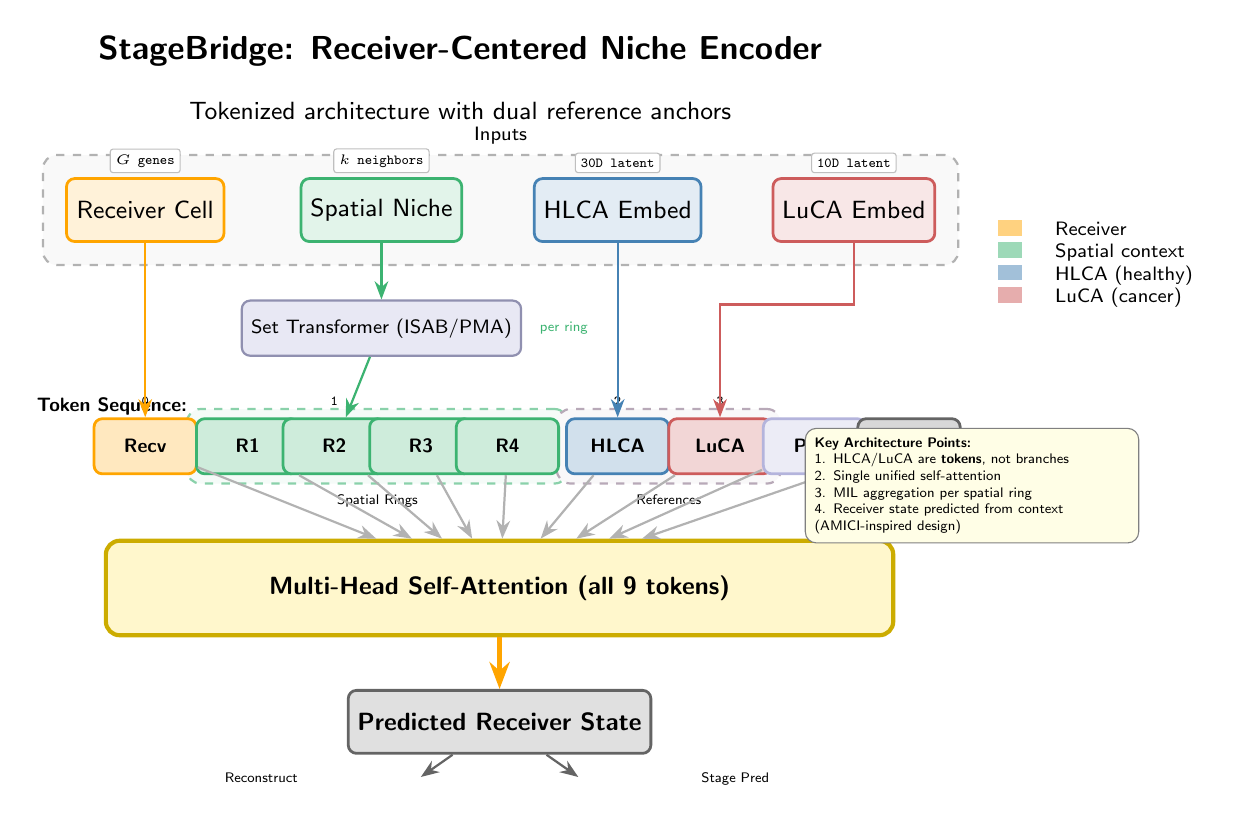
\begin{tikzpicture}[
    % Node styles
    input/.style={
        rectangle,
        draw=#1,
        fill=#1!15,
        rounded corners=3pt,
        minimum width=2cm,
        minimum height=0.8cm,
        font=\small\sffamily,
        line width=1pt
    },
    token/.style={
        rectangle,
        draw=#1,
        fill=#1!25,
        rounded corners=3pt,
        minimum width=1.3cm,
        minimum height=0.7cm,
        font=\scriptsize\sffamily\bfseries,
        line width=1pt
    },
    milblock/.style={
        rectangle,
        draw=milcolor!80!black,
        fill=milcolor!30,
        rounded corners=3pt,
        minimum width=2cm,
        minimum height=0.7cm,
        font=\scriptsize\sffamily,
        line width=0.8pt
    },
    attnblock/.style={
        rectangle,
        draw=attentioncolor!80!black,
        fill=attentioncolor!20,
        rounded corners=5pt,
        minimum width=10cm,
        minimum height=1.2cm,
        font=\small\sffamily\bfseries,
        line width=1.5pt
    },
    output/.style={
        rectangle,
        draw=outputcolor,
        fill=outputcolor!20,
        rounded corners=3pt,
        minimum width=2.5cm,
        minimum height=0.8cm,
        font=\small\sffamily\bfseries,
        line width=1pt
    },
    arrow/.style={
        ->,
        >=Stealth,
        line width=0.8pt,
        #1
    },
    dimbox/.style={
        rectangle,
        draw=gray!50,
        fill=white,
        rounded corners=1pt,
        font=\tiny\ttfamily,
        inner sep=2pt
    },
    groupbox/.style={
        rectangle,
        draw=#1!60,
        fill=#1!5,
        rounded corners=5pt,
        dashed,
        line width=0.8pt
    }
]

% Title
\node[font=\large\sffamily\bfseries, anchor=south] at (0, 6.2)
    {StageBridge: Receiver-Centered Niche Encoder};
\node[font=\small\sffamily, anchor=north] at (0, 6)
    {Tokenized architecture with dual reference anchors};

% ============================================
% INPUT LAYER
% ============================================
\node[input=receivercolor] (receiver_in) at (-4, 4.5) {Receiver Cell};
\node[input=nichecolor] (spatial_in) at (-1, 4.5) {Spatial Niche};
\node[input=hlcacolor] (hlca_in) at (2, 4.5) {HLCA Embed};
\node[input=lucacolor] (luca_in) at (5, 4.5) {LuCA Embed};

% Dimension annotations
\node[dimbox, above=0.05cm of receiver_in] {$G$ genes};
\node[dimbox, above=0.05cm of spatial_in] {$k$ neighbors};
\node[dimbox, above=0.05cm of hlca_in] {30D latent};
\node[dimbox, above=0.05cm of luca_in] {10D latent};

% ============================================
% MIL AGGREGATION (for spatial rings)
% ============================================
\node[milblock] (mil) at (-1, 3) {Set Transformer (ISAB/PMA)};
\node[font=\tiny\sffamily, nichecolor, right=0.1cm of mil] {per ring};

\draw[arrow=nichecolor] (spatial_in) -- (mil);

% ============================================
% TOKEN GENERATION
% ============================================
\node[font=\scriptsize\sffamily\bfseries, anchor=west] at (-5.5, 2) {Token Sequence:};

% 9 tokens
\node[token=receivercolor] (t0) at (-4, 1.5) {Recv};
\node[token=nichecolor] (t1) at (-2.7, 1.5) {R1};
\node[token=nichecolor] (t2) at (-1.6, 1.5) {R2};
\node[token=nichecolor] (t3) at (-0.5, 1.5) {R3};
\node[token=nichecolor] (t4) at (0.6, 1.5) {R4};
\node[token=hlcacolor] (t5) at (2, 1.5) {HLCA};
\node[token=lucacolor] (t6) at (3.3, 1.5) {LuCA};
\node[token=milcolor] (t7) at (4.5, 1.5) {Path};
\node[token=outputcolor] (t8) at (5.7, 1.5) {Stats};

% Type labels
\node[font=\tiny\ttfamily, above=0.02cm of t0] {0};
\node[font=\tiny\ttfamily, above=0.02cm of t2] {1};
\node[font=\tiny\ttfamily, above=0.02cm of t5] {2};
\node[font=\tiny\ttfamily, above=0.02cm of t6] {3};

% Connections to tokens
\draw[arrow=receivercolor] (receiver_in) -- (t0);
\draw[arrow=nichecolor] (mil) -- (t2);
\draw[arrow=hlcacolor] (hlca_in) -- ++(0, -1.2) -| (t5);
\draw[arrow=lucacolor] (luca_in) -- ++(0, -1.2) -| (t6);

% ============================================
% SELF-ATTENTION
% ============================================
\node[attnblock] (attn) at (0.5, -0.3) {Multi-Head Self-Attention (all 9 tokens)};

% Connect tokens to attention
\foreach \tok in {t0, t1, t2, t3, t4, t5, t6, t7, t8} {
    \draw[arrow=gray!60] (\tok) -- (attn);
}

% ============================================
% OUTPUT
% ============================================
\node[output] (out) at (0.5, -2) {Predicted Receiver State};
\draw[arrow=receivercolor, line width=1.5pt] (attn) -- (out);

% Output heads
\node[font=\tiny\sffamily, below left=0.1cm and 0.5cm of out] {Reconstruct};
\node[font=\tiny\sffamily, below right=0.1cm and 0.5cm of out] {Stage Pred};
\draw[arrow=outputcolor] (out) -- ++(-1, -0.7);
\draw[arrow=outputcolor] (out) -- ++(1, -0.7);

% ============================================
% GROUPINGS
% ============================================
\begin{scope}[on background layer]
    \node[groupbox=gray, fit=(receiver_in)(spatial_in)(hlca_in)(luca_in),
          inner sep=8pt, label={[font=\scriptsize\sffamily]above:Inputs}] {};

    \node[groupbox=nichecolor, fit=(t1)(t2)(t3)(t4),
          inner sep=3pt, label={[font=\tiny\sffamily]below:Spatial Rings}] {};

    \node[groupbox=hlcacolor!50!lucacolor, fit=(t5)(t6),
          inner sep=3pt, label={[font=\tiny\sffamily]below:References}] {};
\end{scope}

% ============================================
% LEGEND
% ============================================
\node[anchor=north west, font=\scriptsize\sffamily] at (6.5, 4.5) {
    \begin{tabular}{cl}
        \tikz\fill[receivercolor!50] (0,0) rectangle (0.3,0.2); & Receiver \\
        \tikz\fill[nichecolor!50] (0,0) rectangle (0.3,0.2); & Spatial context \\
        \tikz\fill[hlcacolor!50] (0,0) rectangle (0.3,0.2); & HLCA (healthy) \\
        \tikz\fill[lucacolor!50] (0,0) rectangle (0.3,0.2); & LuCA (cancer) \\
    \end{tabular}
};

% Key insight
\node[rectangle, draw=black!50, fill=yellow!10, rounded corners,
      font=\tiny\sffamily, text width=4cm, align=left] at (6.5, 1) {
    \textbf{Key Architecture Points:}\\
    1. HLCA/LuCA are \textbf{tokens}, not branches\\
    2. Single unified self-attention\\
    3. MIL aggregation per spatial ring\\
    4. Receiver state predicted from context\\
    (AMICI-inspired design)
};

\end{tikzpicture}
\end{document}
